\documentclass[border=7pt]{standalone}
%\documentclass{article}
\usepackage{tikz}
\begin{document}

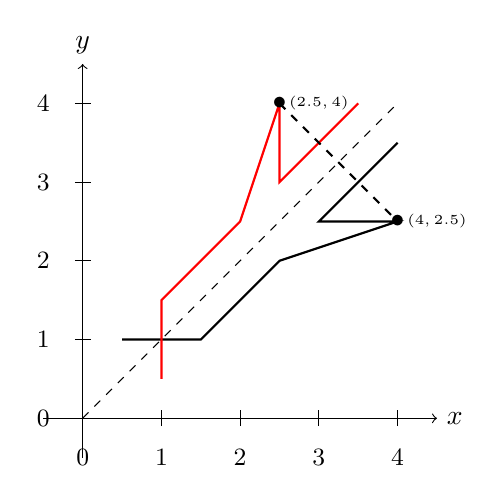
\begin{tikzpicture}

\draw[ thick] (0.5,1) -- (1.5,1)-- (2.5,2)-- (4,2.5) --(3,2.5)--(4,3.5);
\draw[ thick, red] (1, 0.5) -- (1,1.5)-- (2,2.5)-- (2.5,4)-- (2.5,3)--(3.5,4);
\draw[dashed, thick] (2.5,4)--(4,2.5);
\node (c) at (2.5,4) {$\bullet$};
\node (c) at (3,4) {\tiny $(2.5 , 4)$};
\node (c) at (4,2.5) {$\bullet$};
\node (c) at (4.5,2.5) {\tiny $(4, 2.5)$};
% \draw[domain=0:4, smooth, variable=\x,red] plot({\x},{-\x^0.5});

\draw [dashed] (0,0) -- (4,4);
\draw[->] (-0.5,0) -- (4.5,0) node[right] {$x$};
\draw[->] (0,-0.5) -- (0,4.5) node[above] {$y$};

\foreach \x in {0,1,2,3,4}{
     \draw (\x,-0.5) node{\small\x};
     \draw (\x,-0.1) -- (\x,0.1);
     };

\foreach \x in {0,1,2,3,4}{
  \draw (-0.5,\x) node{\small\x};
  \draw (-0.1,\x) -- (0.1,\x);
  };

\end{tikzpicture}
\end{document}
